%
% A Real Chapter
\begin{document}
\chapter{Modeling of directional drilling systems}\label{chapter:Modeling}

In this chapter, several models of a directional drilling system found in literature are presented. Since the main goal of the subsequent research is to develop a controller for this type of systems, models used to develop control strategies are primarily taken into account. In this regard, it has been shown in previous works~\cite{Perneder2013}, that the predominant element in the borehole evolution is the \acs{BHA}; therefore, the models to be considered mainly describe the behavior of the BHA section of the drillstring and its relation with the bit, rock formation and the interface with the forces at the upper part of the drillstring.

The chapter is divided in two main sections: one on numerical and input-ouput correlation models, and the other on first principles models. The first section is aimed to give an overview of finite element and finite difference models found to be used with the purpose of comparing analytical models as well as reviewing input-output correlation models used to develop controllers. The second section of the chapter is focused on so-called first principles models, which describe the behavior of the \acs{BHA} based on physical laws. The models described in this section were chosen to be the most relevant for controller design, despite the fact that it is known that other models also exist.

\section{Numerical and input-output correlation models}\label{section:NumModels}

As directional drilling technology arose, the need to describe its behavior and predict the trajectories that a borehole would take became more important due to the fact that in order to achieve a desired trajectory, experience of the driller was fundamental. This imposed a "trial and error" approach to the process. To overcome this problem, the most common way to assess the issue was to obtain a numerical model for the borehole propagation. 

The works of~\cite{Call81},~\cite{Mill82} and~\cite{Rafi88} are a few examples where finite element methods, combined sometimes with finite difference methods to solve the differential equations that describe the model were used. Nevertheless, these examples do not contain crucial information related to the development of controllers, since most of the properties of the borehole propagation phenomena are not described in detail.

In recent years, Schlumberger\textsuperscript{\textregistered} developed a finite element analysis model called "ST2", made to calculate trajectories of wells formed using a defined \acs{BHA}, a bit and steering unit forces~\cite{Matheus2014}. This model has been mainly used to compare the prediction of the borehole evolution from first principle models such as~\cite{Down07}, showing in~\cite{Downton2011} a good match between the two models. Nevertheless the "ST2" model has not been directly used to develop control algorithms. Due to to the complexity in finite element models, stability analysis and the influence of inputs over the forces and moments acting on the system is not as evident as in first principles models, which makes the latter type more suitable for control. Furthermore, in numerical models the computational effort to predict forces and moments is much greater; this also contributes to the preference of first principle models.

A different type of models to finite element analysis and first principle models are the ones based on input-output correlations, for example neural-networks or polynomial correlations. These models are used to implement controllers in~\cite{Matheus2014}. Since the circumstances where directional drilling systems are used may vary (due to factors such as type of soil, task to be performed, BHA configuration), the development of these type of models is not general since it is based on experimental data, meaning that a model should be build from scratch for every situation.

 Furthermore, these models are generally complex and the inner physical effects in the system are not evident. Because of these reasons, it becomes difficult to perform stability and performance analysis. Finally, in the case of the controller developed in~\cite{Matheus2014}, there is no clear explanation about the behavior and the influence of forces in the model or the controller itself. Due to this, the controllers developed using this type of models are not considered in further sections.

\section{Models based on first principles}

This section is focused on explaining the models that analyze the behavior of the borehole during the directional drilling process based on physical principles. In Subsection~\ref{subsection:Kinematic} describes two types of kinematic models that disregard the effect of the forces on the BHA. 

The last three subsections, describe models given by delay differential equations, which are the most commonly found in literature. The models presented here, were chosen based on the fact that controllers were developed for them.

 Subsection~\ref{subsection:Downton}, outlines the model given in~\cite{Down07}, one of the most common approaches found to be used for controller design in the literature. Subsection~\ref{subsection:Neubert} refers to the model developed in~\cite{Neub97}, which is one of the most important since it included along with the delayed nature of the phenomena, a more detailed bit/rock interaction. Subsection~\ref{subsection:PD} describes the model given in~\cite{Perneder2013}, which makes it interesting since it takes into account the elements given in~\cite{Neub97} and in recent works suitable representation for controller design have been made (\cite{Kremers2013} and \cite{Monsieurs2015}).

\subsection{Kinematic models}\label{subsection:Kinematic}

\paragraph{Kinematic coordinate system transformation.}
One of the approaches found in literature for the modeling of directional drilling systems is the one taken in~\cite{Panchal2010}, where the effects of lateral and torsional forces on the \acs{BHA} and the drillstring are disregarded, considering that they are much faster than the borehole propagation. It is stated, that this assumption is valid for push-the-bit systems, due to the fact that the actuator pushes directly to the wall of the borehole, which gives a high bandwidth to the actuator dynamics. In the case of point the bit systems, the bandwidth of actuator dynamics can be of a similar order to the borehole evolution dynamics, since the toolface (orientation of the drillstring) response is slow because the tool has to cut laterally as it is pointed to the desired direction.

\begin{figure}[ht]\centering
	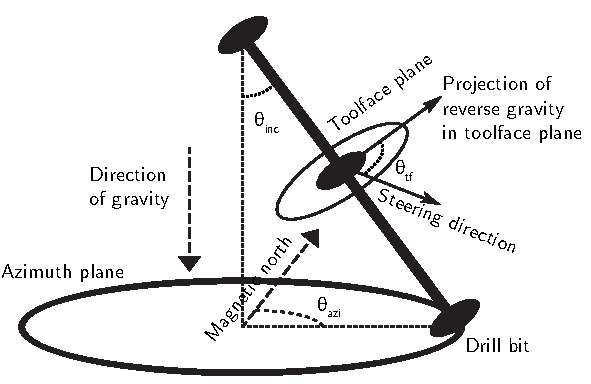
\includegraphics[width=0.5\textwidth]{img/reference.pdf}
	\caption{\label{fig:referenceP}Parameters for BHA~\cite{Panchal2012}.}
\end{figure}

In order to obtain the model, Figure~\ref{fig:referenceP} shows the scheme from which the parameters of the \acs{BHA} are obtained. With these, 5 coordinate frames \lsymb{$F_i$}{Reference frame $i$ in kinematic model for push-the-bit systems.} are defined:

\begin{enumerate}
	\item $F_1$ is the earth frame. Azimuth and inclination angles are defined in this frame and the $x$ vector of the basis is pointing in the direction of gravity, $y$ is perpendicular to $x$ and $z$ completes the frame as a right-handed system.
	\item $F_2$ is the sensor frame which moves along with the drill and represents the direction to which the sensors (accelerometers and magnetometers transducers) are pointing. The $x$ vector of this frame is aligned with the centerline of the borehole and vectors $y$ and $z$ are perpendicular to $x$ rotating with the drill.
	\item $F_3$ is the drill body frame, for this frame the $y$ axis represents $0\degree$ toolface angle. The $x$ axis is the same as $F_2$ and $y$ is perpendicular to $x$ pointing in the direction where an accelerometer would show minimum gravity and $z$ completes the frame as a right-handed system.
	\item $F_4$ is the frame that represents the rotation due to the toolface angle around the $x$ axis of $F_3$, so both $x$ axes are coincidental, $y$ points in the direction of lateral propagation confining the motion of the drill to 2D, and $z$ completes the frame as a right-handed system.
	\item $F_5$ represents the new body axis and is obtained from a rotation around de $z$ axis of $F_4$ by a deflection angle \gsymb{$\theta_{df}$}{Deflection angle in kinematic model for push-the-bit systems.}.
\end{enumerate}

Figure~\ref{fig:Frames} depicts the frames. It has to be noticed that for clarity, frames $F_3$ and $F_4$ are in a different location from $F_2$, in theory this frames have the same origin. Furthermore, frame $F_5$ is not shown but only the angle $\theta_{df}$.

\begin{figure}[ht]\centering
	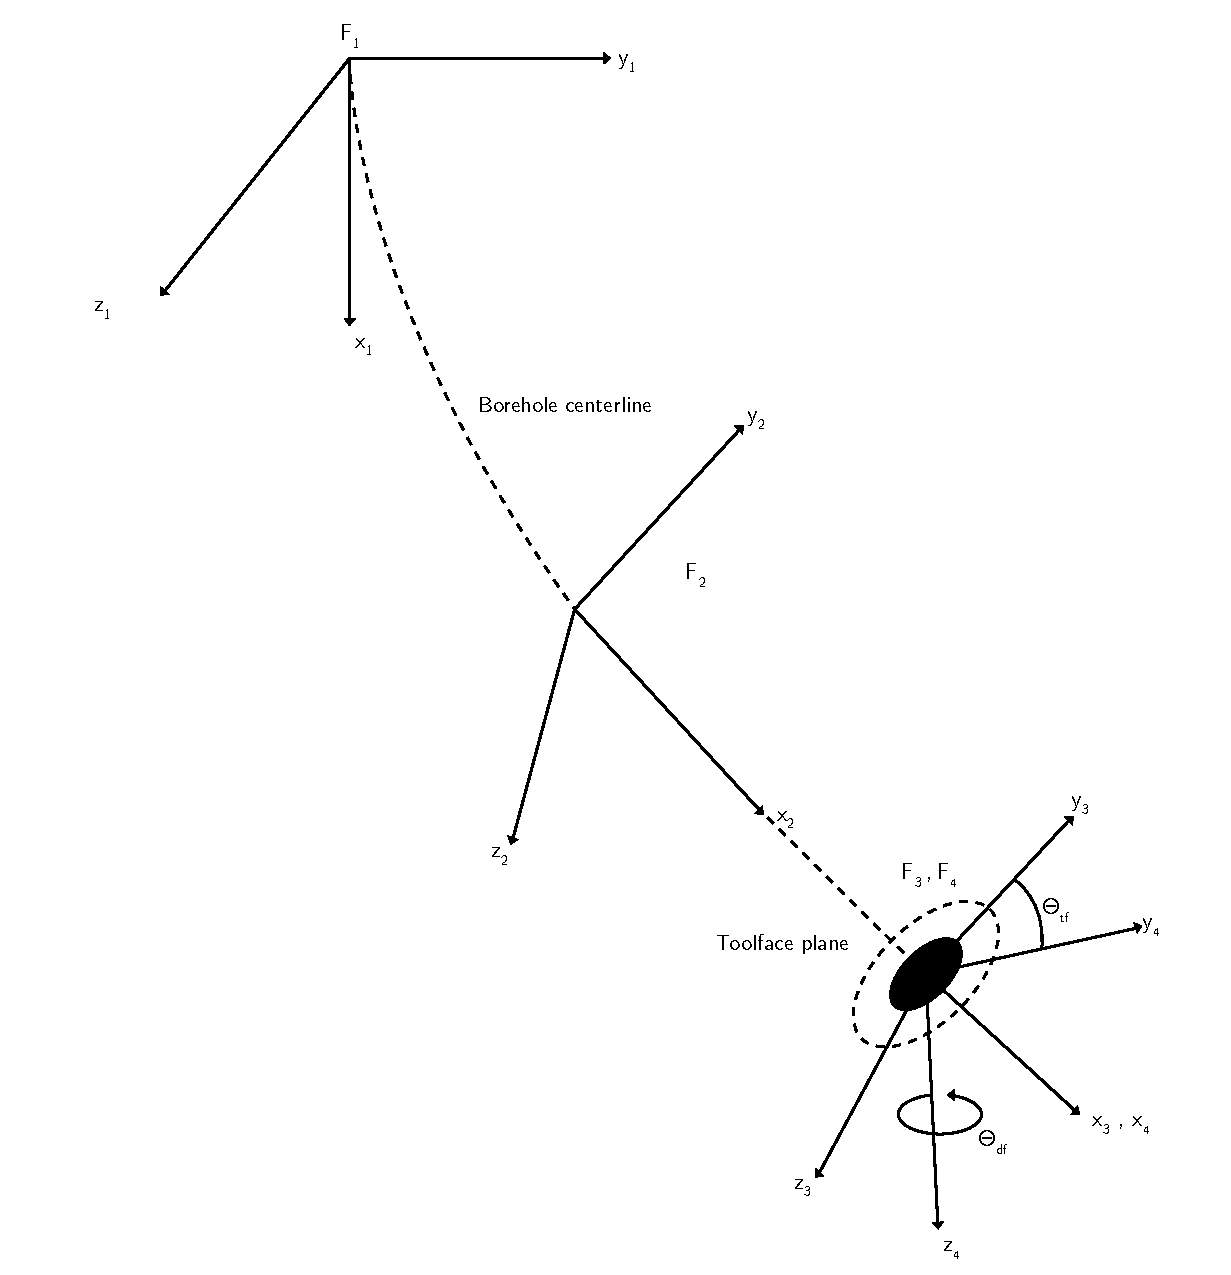
\includegraphics[width=0.5\textwidth]{img/FramesPanchal.pdf}
	\caption{\label{fig:Frames}Frames for kinematic model.}
\end{figure}

Using these definitions, the coordinates of the body frame $F_3$ with respect to the earth frame are obtained through the direction cosine matrices $R_{inc}$ and $R_{azi}$ by:

\begin{equation}
F_3 = R_{inc}R_{azi}F_1,
\end{equation}

where the matrices \lsymb{$R_{inc}$}{Direction cosine matrix with respect to the inclination angle in kinematic model for push the bit systems.} and \lsymb{$R_{azi}$}{Direction cosine matrix with respect to the azimuth angle in kinematic model for push-the-bit systems.} are defined by:

\begin{align*}
	R_{inc} = 
	\begin{bmatrix}
		\cos{\theta_{inc}} & \sin{\theta_{inc}} & 0 \\
		-\sin{\theta_{inc}} & \cos{\theta_{inc}} & 0 \\
		0 & 0 & 1
	\end{bmatrix}, \qquad
	R_{azi} = 
	\begin{bmatrix}
	1 & 0 & 0 \\
	0 & \cos{\theta_{azi}} & \sin{\theta_{azi}} \\
	0 & -\sin{\theta_{azi}} & \cos{\theta_{azi}}
	\end{bmatrix}, 	
\end{align*}

with \gsymb{$\theta_{inc}$}{Inclination angle in kinematic model for push-the-bit systems.} and \gsymb{$\theta_{azi}$}{Azimuth angle in kinematic model for push-the-bit systems.} the inclination and azimuth angles, respectively.

Subsequently, the attitude is defined as the unit vector aligned in the direction where the drill is pointing, which is the same direction as the $x$ axis of frame $F_3$ defined as:
\begin{equation}
	x_{F_3}=R_{inc}R_{azi}x_{F_1},
\end{equation}

where $x_{F_1}$ and $x_{F_3}$ are the vectors pointing in the direction of $x$ at time t in frames $F_1$ and $F_3$, respectively. 

After this definition, the defined attitude is perturbed in order to achieve a new orientation at time $t + \delta t$, which is done with two different methods. In the first method, two infinitesimal rotations $dR_{inc}$ and $R_{inc}dR_{azi}R_{inc}^{-1}$ are applied to the basis in the following way:

\begin{equation}
	x_{F_3}=dR_{inc}R_{inc}dR_{azi}R_{inc}^{-1}x_{F_3}',
	\label{eq:attituded}
\end{equation}

where $x_{F_3}'$ is the $x$ vector of frame $F_3$ at time $t+\delta t$.
The azimuth infinitesimal rotation has to be transformed to the same basis as the previous rotation. Therefore it is multiplied by the rotation matrix of the inclination and its inverse. Due to small angle approximations, the infinitesimal rotation matrices $dR_{inc}$ and $dR_{azi}$ are defined as:

\begin{gather*}
	dR_{inc} = 
	\begin{bmatrix}
	1 & d\theta_{inc} & 0 \\
	-d\theta_{inc} & 1 & 0 \\
	0 & 0 & 1
	\end{bmatrix}, \qquad
	dR_{azi} = 
	\begin{bmatrix}
	1 & 0 & 0 \\
	0 & 1 & d\theta_{azi} \\
	0 & -d\theta_{azi} & 1
	\end{bmatrix} .	
\end{gather*}

Performing the matrix multiplications, Equation (\ref{eq:attituded}) is:


\begin{equation}
	x_{F_3}=\begin{bmatrix}
	1 & d\theta_{inc} & -(\sin{\theta_{inc}} + d\theta_{inc}\cos{\theta_{inc}}) d\theta_{azi} \\
	-d\theta_{inc} & 1 & -(\cos{\theta_{inc}} + d\theta_{inc}\sin{\theta_{inc}}) d\theta_{azi} \\
	d\theta_{azi}\sin{\theta_{inc}} & d\theta_{azi}\cos{\theta_{inc}} & 1
	\end{bmatrix} 
			x_{F_3}'.
	\label{eq:attitudedd}
\end{equation}

Since $ d\theta_{azi} d\theta_{inc}$ is negligible (in a first order approximation), and for a given $x_{F_3} = (1,0,0)^T$, the position of the new body axis with respect to the current body axis in terms of infinitesimal displacements of azimuth and inclination of the attitude is:

\begin{equation}
	x_{F_3}' = 
				\begin{bmatrix}
				1 \\
				d\theta_{inc}\\
				-\sin{\theta_{inc}}d\theta_{azi}
				\end{bmatrix}.
\end{equation}

The second method uses an infinitesimal deflection angle $\theta_{df}$. This is done by moving from frame $F_3$ to frame $F_4$, where the $y$ axis is rotated clockwise about the $x$ axis by an angle of $\theta_{tf}$. Now from the $F_4$ frame, a rotation of the deflection angle about the $z$ axis will give the required transformation:

\begin{equation}
	x_{F_3} = R_{df} R_{tf} x_{F_3}',
\end{equation}

where the rotation matrices \lsymb{$R_{df}$}{Rotation matrix with respect to the deflectoin angle in kinematic model for push-the-bit systmms.} and \lsymb{$R_{tf}$}{Rotation matrix with respect to the toolface angle in kinematic model for push-the-bit systems.} are defined by:

\begin{gather*}
	R_{df} = 
	\begin{bmatrix}
		1 & d\theta_{df} & 0 \\
		-d\theta_{df} & 1 & 0 \\
		0 & 0 & 1
	\end{bmatrix}, \qquad
	R_{tf} = 
	\begin{bmatrix}
		1 & 0 & 0 \\
		0 & \cos{\theta_{tf}} & \sin{\theta_{tf}} \\
		0 & -\sin{\theta_{tf}} & \cos{\theta_{tf}}
	\end{bmatrix} ,	
\end{gather*}

and in the same fashion as in the previous method, for a given attitude $x_{F_3} = (1,0,0)^T$ the new position is given by:

\begin{equation}
	x_{F_3}' = 
		\begin{bmatrix}
		1 \\
		d\theta_{df}\cos{\theta_{tf}}\\
		-d\theta_{df}\sin{\theta_{tf}}
	\end{bmatrix}.
\end{equation}

Since the attitudes in method 1 and 2 are equivalent, then it can be said:

\begin{align}\label{eq:2methods}
	d\theta_{inc}  &= d\theta_{df}\cos{\theta_{tf}}, \nonumber \\
	\sin{\theta_{inc}}d\theta_{azi} &= d\theta_{df}\sin{\theta_{tf}}.
\end{align}

Finally as $d\theta_{df}$ is a deflection angle in the lateral direction in which the tool is propagating, it can be defined as:

\begin{equation}\label{eq:dtheta}
	d\theta_{df} = V_{rop}K_{dls}\delta t,
\end{equation}

where \lsymb{$V_{rop}$}{Rate of penetration in kinematic model for push-the-bit systems.} is the rate of penetration, \lsymb{$K_{dls}$}{Maximum curvature response of kinematic model for push-the-bit systems.} is the maximum curvature response, which is used because most of the drilling tools can only respond with this value. By replacing Equation (\ref{eq:dtheta}) in (\ref{eq:2methods}), and taking the limit that $\delta t$ is small, the inclination and azimuth equations are given by:

\begin{align}
\frac{d\theta_{inc}}{dt} & =  V_{rop} K_{dls} \cos{\theta_{tf}}, \\
\sin{\theta_{inc}} \frac{d\theta_{azi}}{dt} & =  V_{rop} K_{dls} \sin{\theta_{tf}},
\end{align}

Since the drill is always responding with $K_{dls}$, to generate curvatures smaller than this value the tool is made to drill in drilling cycles. This is similar to the duty cycles used in electronics for pulse-width modulation. By using drilling cycles, curvatures between 0 and $K_{dls}$ can be obtained. The percentage between the maximum curvature is called steering ratio. $K_{dls}$ can be replaced for \lsymb{$U_{dls}$}{Dog leg severity or curvature in kinematic model for push-the-bit systems.}, which is the curvature or the so-called "dog leg severity", defined as the steering ratio times $K_{dls}$. With these considerations, the previous equations can be rewritten as: 
 

\begin{align}
	\dot{\theta}_{inc} & =  V_{rop} U_{dls} \cos{U_{tf}}\label{eq:KinMod1}, \\
	\dot{\theta}_{azi} & =  \frac{V_{rop}}{\sin{\theta_{inc}}} U_{dls} \sin{U_{tf}}\label{eq:KinMod2},
\end{align}

where \lsymb{$U_{tf}$}{Toolface control input in kinematic model for push-the-bit systems.} is the toolface angle control input. It can be seen that both equations are coupled due to the toolface angle. The following input transformation is proposed:

\begin{align}
	U_{tf} &=  \arctan{\frac{U_{azi}}{U_{inc}}}\label{eq:InputTransPan1}, \\
	U_{dls} &= K_{dls}\sqrt{(U_{azi})^2 + (U_{inc})^2}\label{eq:InputTransPan2},
\end{align}

where \lsymb{$U_{inc}$}{Virtual control input for the inclination in the kinematic model for push-the-bit system.} and \lsymb{$U_{azi}$}{Virtual control input for the azimuth in the kinematic model for push-the-bit system.} are virtual control inputs for inclination and azimuth. These equations are valid since $U_{tf}$ and $U_{dls}$ are control inputs to the system and $K_{dls}$ can be taken as a given constant parameter. From Equation (\ref{eq:InputTransPan1}) can be deduced:

\begin{align*}
	\tan{U_{tf}} =  \frac{U_{azi}}{U_{inc}} = \frac{\sin{U_{tf}}}{\cos{U_{tf}}}, \\
	\sin{U_{tf}}^2 + \cos{U_{tf}}^2 = 1.
\end{align*}

If we substitute the input transformations in Equations (\ref{eq:KinMod1}) and (\ref{eq:KinMod2}) the resulting kinematic model is:

\begin{align}
	\dot{\theta}_{inc} & =  V_{rop} K_{dls} U_{inc}\label{eq:nonlinearPanchal1}, \\
	\dot{\theta}_{azi} & =  \frac{V_{rop}}{\sin{\theta_{inc}}} K_{dls} U_{azi}\label{eq:nonlinearPanchal2}.
\end{align}

The latter set of equations shows an input decoupling between both expressions. Nevertheless, the inclination angle is still present in the derivative of the azimuth.

A final remark is important to be made about this model related to the sensor positioning. It is stated that the tool is equipped with its own attitude sensor which gives measurements of azimuth and inclination, but that the sensor data is not spatially coincidental with the inertial data (i.e. the location of the sensors is not at where the tool is placed). This situation is taken into account by using time delays via Padé approximations.

\paragraph{Rigid rod hinged model.}
The parameters for this model are given in Figure~\ref{fig:referenceP} as well. Despite this, the main difference lies in the fact that the system is modeled as a hinge, similar to a robotic system, with a rotational motion only corresponding to pitch and yaw~\cite{Panchal2012}.  To obtain the evolution of the attitude with respect to time, first the attitude of the bit with respect to the earth frame can be expressed as:

\begin{equation}
	x^j = R_i^j x^i,
\end{equation}
 
 where $x^i$ is the attitude of the body expressed in its own frame, $x^j$ is the attitude of the body expressed in the earth frame and $R_i^j$ is the rotation matrix from the body frame to the earth frame. If the derivative of the attitude is obtained the result is:
 
 \begin{equation}
 	\dot{x}^j = \dot{R}_i^jx^i
 	\label{eq:dotx}.
 \end{equation}
 
In order to continue with the derivation, the tilde operator needs to be introduced. Consider the angular velocity vector $\omega = \begin{bmatrix}\omega_1 & \omega_2 & \omega_3\end{bmatrix}^T$. The tilde operator is defined as:

\begin{equation*}
	\tilde{\omega} = 
	\begin{bmatrix}
		0 & -\omega_3 & \omega_2 \\
		\omega_3 & 0 & -\omega_1 \\
		-\omega_2 & \omega_1 & 0
	\end{bmatrix}.
\end{equation*}
 
Furthermore, the matrices to rotate frames in a three-dimensional space belong to the rotation group SO(3), which yields the following property:

\begin{equation*}
	R^T R = I.
\end{equation*}

If then the derivative of this expression is calculated, we obtain the following property:

 \begin{equation*}
 	\dot{R}^TR = -(\dot{R}^TR)^T.
 \end{equation*}
 
 This implies that the matrix $\dot{R^T}R$ is skew symmetric and the same can be proven for $\dot{R}R^T$. Using this property, a variant of the Poisson equation can be written, so in the case of $\omega$ in the body frame (in the case of a directional drilling system is the frame located at the bit) this results in:
 
 \begin{equation}
 	\tilde{\omega} = \dot{R}_i^j R_j^i
 	\label{eq:omega}.
 \end{equation}
 
 If we substitute $\dot{R_i}$ from Equation (\ref{eq:omega}) in Equation (\ref{eq:dotx}) then the expression for the evolution of the attitude can be expressed as:
 
 \begin{equation}
 	\dot{x}^j = \tilde{\omega}x^j.
 \end{equation}
 
 It should be noticed, that if a tilde matrix is multiplied by a vector, the result is equivalent to:
 
  \begin{equation*}
  \dot{x}^j = \omega \times x^j.
  \end{equation*}
  
  In this model, the angular velocity vector $\omega$ is the input of the system. This is similar to a robotic system where the control inputs are the angular velocities of the motors on each joint. The vector $x$ represents the attitude of the tool, which is defined in a similar way as in the previous model, being the $x$ vector of the frame fixed to the tool position.
 
Therefore, if only rotation is considered, the evolution in time of the attitude can be described as in Figure~\ref{fig:pointkmodel}.

\begin{figure}[ht]\centering
	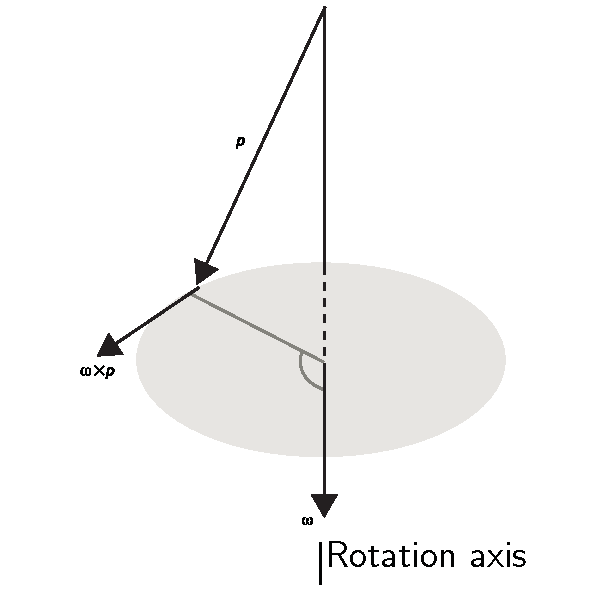
\includegraphics[width=0.5\textwidth]{img/rotationkin.pdf}
	\caption{\label{fig:pointkmodel}Kinematic point-the-bit model.}
\end{figure}

The two kinematic models present a very simple description of the directional drilling system, due to the fact that it disregards the dynamic effects on the BHA. This simplicity provides the advantage that several type of conventional methods for controller design can be applied. Despite this, since the model has not yet been validated with field or experimental data, it can not be proven that the considered assumptions hold in general. Besides, as it will be mentioned in further sections, the models that use delay differential equations and take into account forces and moments of the system, present a good match with both numerical and experimental data, which can lead to the conclusion that this effects are important to borehole evolution.

\subsection{\acf{EFFSZM} model}\label{subsection:Downton}

This model was developed by Downton in~\cite{Down07}. The derivation of this model comes from two previous representations with certain assumptions to simplify the effects present in directional drilling. These two models are the \acf{ISISZM} and the \acf{FSFSZM} drilling systems~\cite{Down07}. 

Figure~\ref{fig:downton} shows the directional drilling system. The independent variable of the system is distance drilled and the actuator force is placed at a distance $a$ from the drill bit, which applies force to the walls of the borehole in order to steer the drillstring (similar to a push-the-bit system). The first stabilizer is positioned at a distance $b$ from the bit. Coordinate $m-c$ yields the position of a \textit{flex-joint}, similar to a hinge to simulate a \textit{lumped} compliance. Finally at distance $d$ an upper stabilizer is placed.

\begin{figure}[ht]\centering
	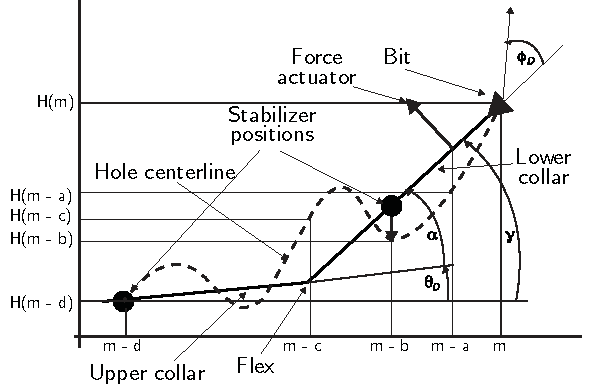
\includegraphics[width=0.6\textwidth]{img/Downtonmodel.pdf}
	\caption{\label{fig:downton}Flex-hinge directional drilling system~\cite{Down07}.}
\end{figure}

The borehole centerline is represented by function \lsymb{$H(m)$}{Borehole centerline in EFFSZM model.} and all angles are assumed to be small assuming that axis $m$ is approximately aligned to the direction of drilling. Angle \gsymb{$\phi_{D}$}{Direction of drilling in EFFSZM model.} represents the direction to which the borehole is propagating with respect to the lower collar axis, as shown in Figure~\ref{fig:downton}. Furthermore, the borehole-propagation angle with respect to the $m$ axis is given by $\frac{dH}{dm}$, \gsymb{$\alpha$}{Orientation of upper collar with respect to the lower collar in EFFSZM model.}  represents the orientation of the upper collar with respect to the lower collar and \gsymb{$\theta_D$}{Orientation of upper collar with respect to $m$ EFFSZM model.} represents the orientation of the lower collar with respect to the $m$ axis. Then, the propagation angle at the bit can be written as:

\begin{equation}
	\frac{dH}{dm} = \phi_D + \alpha + \theta_D.
	\label{eq:tangent}
\end{equation}

In order to have a useful model for prediction of borehole response, the right-hand side of the equation needs to be expressed in terms of the borehole, steering actuator geometry and the externally applied forces. Initially, it is assumed that the bit cuts laterally at a lateral rate \lsymb{$LROP$}{Lateral rate of penetration in EFFSZM model.} for a lateral weight \lsymb{$LWOB$}{Lateral rock/bit load in EFFSZM model.} and with rotational speed \lsymb{$RPM$}{Rotational speed of the bit EFFSZM model.}. The bit/rock interaction is simplified using a constant, namely \lsymb{$Klat$}{Lateral bit/rock interaction constant in EFFSZM model.}, resulting in the final expression for $LROP$:

\begin{equation}
LROP = LWOB \cdot Klat \cdot RPM.
\end{equation}

It is important to notice, that the symbol "$\cdot$" does not represent the inner product, but it is used in order to be consequent with the authors notation and to avoid confusion between variables. In a similar way, the axial rate of penetration \lsymb{$ROP$}{Axial rate of penetration in EFFSZM model.} is obtained for a given axial load \lsymb{$WOB$}{Axial load in EFFSZM model.} at a rotational speed $RPM$. As before, the bit/rock interaction is lumped into a constant, namely \lsymb{$Klong$}{Axial bit/rock interaction constant in EFFSZM model.} resulting in the expression:

\begin{equation}
	ROP = WOB \cdot Klong \cdot RPM.
\end{equation}
%Here a general outline of this model will be given in order to support the control algorithms developed for this model. The previous works of ~\cite{Downton2011} will be used for this subsection.

With these two expressions, angle $\phi_D$ can be determined by:

\begin{equation}
	\phi_D = \arctan{\bigg( \frac{-LWOB \cdot Klat}{WOB \cdot Klong} \bigg)}
	\label{eq:phiD}.
\end{equation}

It can be noticed that the numerator yields a negative sign, which could be explained by taking the direction of $LROP$ pointing downwards from the bit and perpendicular to the upper collar axis. Since under normal drilling conditions, the axial penetration is much bigger than the lateral penetration, the numerator of (\ref{eq:phiD}) dominates the expression and small-angle assumptions can be made. After force and moment balancing, $LWOB$ is obtained as:

\begin{equation}
	LWOB = \bigg[ \frac{b-d}{b \cdot (c-d)} \cdot Kflex + \frac{b-c}{b} \cdot WOB\bigg] \cdot \alpha + \frac{a-b}{b} \cdot Fpad,
\end{equation}

where \lsymb{$Kflex$}{Angular spring rate of flex joint in EFFSZM model.} is the angular spring rate of the flex joint and \lsymb{$Fpad$}{Force actuator output in EFFSZM model.} is the force actuator input. Finally finding the expressions for angles $\alpha$ and $\theta_D$:

\begin{align}
\alpha + \theta_D &= \frac{H(m) - (H(m-b) - V(m))}{b}, \\
\alpha &= \frac{H(m) \cdot (b - d) + d \cdot (H(m - b) - V(m)) - H(m-d) \cdot b}{b \cdot (c-d)},
\end{align}

where \lsymb{$V(m)$}{Actuator displacement in EFFSZM model.} is the actuator position in terms of $m$, and solving for the borehole tangent defined in (\ref{eq:tangent}) results in:

\begin{align}\label{eq:DowntonModelt}
		\frac{dH}{dm} =& \bigg( \frac{1+Cf}{b}\bigg) \cdot (V(m) - H(m-b)) + \frac{Cf}{d} \cdot H(m-d) \nonumber \\
		 &+ \bigg( \frac{d \cdot (1+Cf) - b}{b \cdot d}\bigg) \cdot H(m) + \frac{(b-a) \cdot Fpad}{b \cdot WOB \cdot Kanis},
\end{align}

where $Cf$ and $Kanis$ are defined as:

\begin{align*}
	Cf =& \bigg(\frac{c-b}{Kanis} - \frac{d-b}{d-c} \cdot \frac{Kflex}{WOB}\bigg) \cdot \frac{d}{b \cdot (d-c)}, \\
	Kanis  =& \frac{Klong}{Klat}.
\end{align*}

It can be seen that the current orientation with respect to $m$ depends on the past orientation, which provides a delayed nature to the system. The model response was compared with the previously mentioned "ST2" model from Schlumberger\textsuperscript{\textregistered} obtaining a good match for certain results~\cite{Down07}. Finally as it is important to get a representation useful for control, the previous set of expression is transformed to the Laplace domain with respect to $m$ as:

\begin{equation}\label{eq:DowntonModel}
	H(s) = \frac{\frac{1+Cf}{b} \cdot V(s) + \frac{(b-a) \cdot Fpad(s)}{b \cdot WOB \cdot Kanis}}{s + \bigg(\frac{Cf}{d} - \frac{(1+Cf)}{b}\bigg) - \frac{Cf}{d} \cdot e^{-sd} + \frac{1+Cf}{b} \cdot e^{-sb}}.
\end{equation}

From this transfer function, if $Fpad(s)$ is taken as input to the system and the derivative of the displacement in the Laplace domain $sH(s)$ is taken as output, a transfer function representation can be obtained.

A great advantage of this model is that its match with an specific numerical model has been tested with promising results. Furthermore, a transfer function representation can be obtained to use as a basis for controller design. Nevertheless, the bit/rock interaction is not as detailed as in other models. Another important aspect lies in the fact that this model has been derived only for a two-dimensional drilling system. This is a major disadvantage since, some of the crucial causes of borehole spiraling take place due to the effects on three dimensions (i.e. bit walk). Finally, the model is derived in terms of deformation from an initial configuration, restricting the model to small angle rotations.

\subsection{Neubert and Heisig model}\label{subsection:Neubert}

This model is considered to be one of the pioneer steps in first-principle-based modeling for directional drilling nowadays. The key elements that were introduced are the use of delay differential equations to describe the borehole evolution, analysis of kinematics and the deduction of a new bit/rock interaction. Despite this, there is only a small number of international publications regarding this model. The most detailed description is given in~\cite{NeubertM.andHeisig1997}. 

\begin{figure}[ht]\centering
	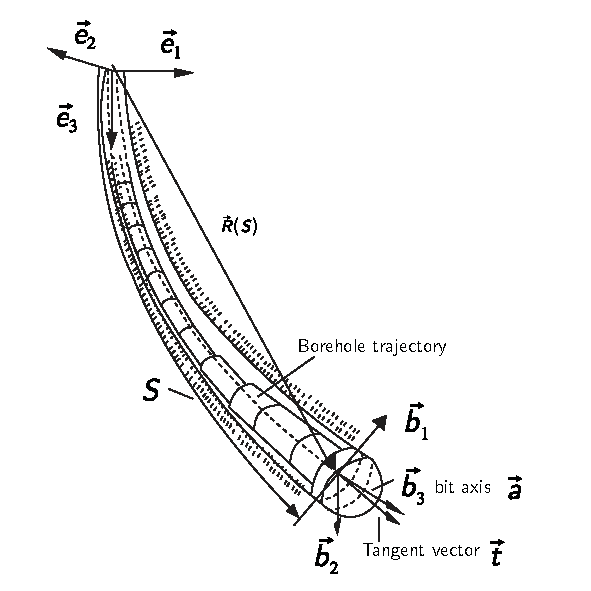
\includegraphics[width=0.5\textwidth]{img/Neubert.pdf}
	\caption{\label{fig:Neubert}Neubert and Heisig geometric description~\cite{NeubertM.andHeisig1997}.}
\end{figure}

\paragraph{Kinematics.}The derivation starts with the kinematics, Figure~\ref{fig:Neubert} shows the parameters of a directional drilling system. The centerline or trajectory is described by vector:

\begin{equation}
\vec{R}(S) = R_1(S) \vec{e}_x + R_2(S) \vec{e}_y + R_3(S) \vec{e}_z = R^T \cdot \vec{\underline{e}},
\end{equation}

where $S$ denotes the measured depth along the trajectory and $R_i(S)$ the coordinates of the point in an earth-fixed coordinate system with respect to the base $\vec{\underline{e}}$. The tangent vector \lsymb{$\vec{t}$}{Tangent vector in Neubert and Heisig model} is given by:

\begin{equation}
	\vec{t} = \vec{R}' = \frac{d\vec{R}}{dS}.
\end{equation}

The interaction between the rock and the bit takes place in the local coordinate system \lsymb{$(\vec{b}_1,\vec{b}_2,\vec{b}_3)$}{Coordinate system for bit/rock interaction in Neubert and Heisig model.} placed at the connection point of the drillstring and the bit. The direction of the bit is defined by vector \lsymb{$\vec{a}$}{Direction of the bit in Neubert and Heisig model.} such that:

\begin{equation}
	\vec{a} = \vec{b}_3.
\end{equation}

Taking into account that the bit axis and the tangent vector $\vec{t}$ of the borehole are not necessarily aligned, the two rotation vectors \gsymb{$\gamma_1$}{Rotation vector 1 in Neubert and Heisig model} and \gsymb{$\gamma_2$}{Rotation vector 2 in Neubert and Heisig model}  are considered in such way that:

\begin{equation}
	\vec{\underline{b}} = \underline{\underline{T}}(\gamma_1,\gamma_2)  \vec{\underline{e}},
\end{equation}

where $\underline{\underline{T}}$ is a transformation matrix for the two rotation angles $\gamma_1$ and $\gamma_2$. Finally it is assumed that the bit rotates with angular velocity $\vec{\Omega}$ and with constant rate of penetration $\vec{v}$. Then the five variables to describe the motion of the bit are: $R_1$, $R_2$, $R_3$, $\gamma_1$ and $\gamma_2$.

\paragraph{Rock/Bit interaction model.} The interaction model is given by describing the force vector $\vec{F}$, the moment vector $\vec{M}$ in terms of the tangent vector $\vec{t}$ and reactive forces and moments related to the change of position of the bit and the rock properties. The following relation is assumed:

\begin{align}
	\vec{F} &= p (\underline{\underline{G}}_A \vec{t} + \underline{\underline{G}}_B \vec{a}),\nonumber \\
	\vec{M} &= p (\underline{\underline{G}}_C \vec{t} + \underline{\underline{G}}_D \vec{a}),
	\label{eq:bitrockneubert}
\end{align}

where the factor $p$ denotes the axial feed per revolution, denoted as $p = 2\pi \vec{v}/\vec{\Omega}$, and \lsymb{$\underline{\underline{G}}_A, \underline{\underline{G}}_B, \underline{\underline{G}}_C, \underline{\underline{G}}_D$}{Coefficient matrices for rock/bit interaction in Neubert and Heisig model.} are formulated in the local bit coordinate system $\vec{b}$ and are given by:

\begin{align}
	\underline{\underline{G}}_j = \begin{bmatrix}
	g_{j11} & g_{j12} & 0 \\
	-g_{j12} & g_{j22} & 0 \\
	0 & 0 & g_{j33}
	\end{bmatrix}, \qquad  \textrm{ for } j = A,B,C,D.
\end{align}

The determination of the matrix coefficients is suggested to be done in two ways: by performing proper experiments and obtaining data to do system parameter identification or by estimating the coefficients by an analysis of the cutting behavior of the bit. The latter alternative was done in~\cite{Neub97} and the obtained coefficients are registered in~\cite{NeubertM.andHeisig1997}.

\paragraph{Drillstring model.}

The model of the drillstring only takes into account the lower part of the BHA, where the upper part transmits both axial load and torsional moment. An important assumption of this model, is the inclusion of a first stabilizer with adjustable eccentricity in order to steer the drill bit, and that there is no radial clearance between the borehole wall and the stabilizers. Finally the system is modeled using Euler-Bernoulli beam theory, resulting in a closed form solution of the system for the forces and moments at the bit.

The equations for the forces and moments at the bit are given by:

\begin{align}
\vec{F} &= f (\vec{r}(S-\sigma),\vec{a},\vec{\varepsilon}), \nonumber\\
\vec{M} &= f (\vec{r}(S-\sigma),\vec{a},\vec{\varepsilon}) ,
\label{eq:BHAneubert}
\end{align}

where the function $\vec{r}$ represents the already drilled trajectory, \gsymb{$\sigma$}{Delay of the drilled trajectory in Neubert and Heisig model.} is a delay in the drilled trajectory and \gsymb{$\vec{\varepsilon}$}{Eccentricity of first stabilizer in Neubert and Heisig model.} is the eccentricity of the first stabilizer. In~\cite{Neub97}, it is stated that function $f$ is nonlinear, although it is not clear where the nonlinearity comes from. Combining Equations (\ref{eq:bitrockneubert}) and (\ref{eq:BHAneubert}) and rearranging the terms results in the differential equation:

\begin{equation}
\underline{\underline{C}}(\underline{z}(S)) \underline{z}'(S) = f(\underline{z}(S), \underline{z}(S-\sigma), \underline{\varepsilon}),
\end{equation}

where the newly introduced vector \lsymb{$\underline{z}(S)$}{Vector of motion variables in Neubert and Heisig model} and its derivative $z'(S)$ contain $R_1$, $R_2$, $R_3$, $\gamma_1$ and $\gamma_2$ and their derivatives with respect to (S), respectively; and matrix $\underline{\underline{C}}$ contains the effects of forces and moments as a function of $z(S)$.

This model yields several advantages with respect to the previously presented ones. First of all, it uses a bit/rock interaction model that takes into account both axial and lateral effects on the bit. Furthermore, the dynamics take into account the delayed nature of the phenomenon and it is modeled for a three-dimensional system. Nevertheless, it is difficult to comprehend the exact mechanisms that have an influence since the international published paper on this model is not detailed enough. As a final remark on this model, the basic principles behind are extended by the PD model, supporting the initial statement of this subsection about its pioneering role in first principle modeling.


\subsection{PD model}\label{subsection:PD}
This model was developed by Perneder and Detournay in~\cite{Perneder2013}, \cite{Perneder2012}, \cite{Perneder2013a} and \cite{Perneder2013b} from where its name comes. As the previous 2 models it is based on delay differential equations. The delayed nature comes from the fact that the drillstring has to fit inside the borehole that has already been drilled. The geometric description for this model is shown in Figure~\ref{fig:geoPD}.

\begin{figure}[ht]\centering
	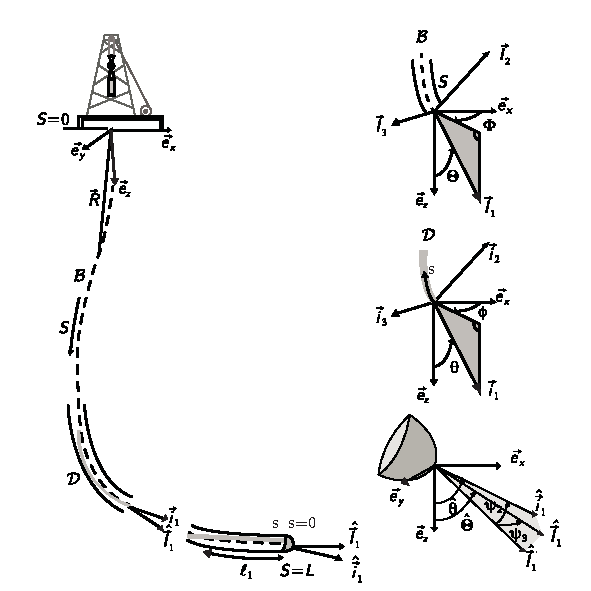
\includegraphics[width=0.6\textwidth]{img/geodesc.pdf}
	\caption{\label{fig:geoPD}Geometric description of directional drilling system.}
\end{figure}

The elements of the geometric description of the model are listed below:
\begin{enumerate}
	\item The fixed coordinate basis is given by \lsymb{$(\vec{e}_x,\vec{e}_y, \vec{e}_z)$}{Fixed coordinate system in the PD/Neubert and Heisig models.}. It is located at the drill rig and vector $\vec{e}_z$ points in the direction of gravity and is perpendicular to $\vec{e}_x$ and $\vec{e}_y$ for a right-handed system. 
	
	\item The borehole is described as a function of the curvilinear coordinate \lsymb{$S$}{Curvilinear coordinate in PD/Neubert and Heisig models.}, with $0 \leq S \leq L$ where $0$ is the value of the coordinate at the surface and \lsymb{$L$}{Total length of borehole in PD model.} is the total length of the borehole.
	
	\item The borehole axis \lsymb{$\mathcal{B}$}{Borehole axis in PD model.} is defined as the trajectory of a reference point at the bit.
	
	\item The vector function \lsymb{$\vec{R}(S)$}{Vector function of borehole axis $\mathcal{B}$ in curvilinear coordinates $S$ in PD/Neubert and Heisig model} for $S \in [0,L]$ describes the borehole axis $\mathcal{B}$ as a function of $S$ in the fixed basis.
	
	\item At a certain position, the direction of the borehole can be locally defined by the tangent vector of the borehole axis $\vec{I}_1 = \frac{d \vec{R}}{d S}$. Using this vector, a local basis \lsymb{$(\vec{I}_1,\vec{I}_2, \vec{I}_3)$}{Basis for the borehole axis in the PD model.} for the borehole can be defined with $\vec{I}_3 \cdot \vec{e}_y = 0$ (parallel) and $\vec{I}_1 \times \vec{I}_2 = \vec{I}_3$ (perpendicular) and defining the frame as right-handed.
	
	\item The borehole inclination \gsymb{$\Theta$}{Borehole inclination in PD model.} is the angle between vector $\vec{e}_z$ and $\vec{I}_1$ as a function of the curvilinear coordinate $S$.
	
	\item The borehole azimuth \gsymb{$\Phi$}{Borehole azimuth in PD model.} is the angle between $\vec{e}_x$ and the projection of $\vec{I}_1$ to the plane spanned by $\vec{e}_x$ and $\vec{e}_y$.
	
	\item The \acs{BHA} axis is described as a function of the curvilinear coordinate $s \in [0,L_{BHA}]$ where $0$ is the position of the drill bit and \lsymb{$L_{BHA}$}{Length of the BHA in PD model.} is the length of the \acs{BHA}.
	
	\item The \acs{BHA} axis \lsymb{$\mathcal{D}$}{BHA axis in PD model.} is considered to be slightly deviated from the borehole axis $\mathcal{B}$ (due to deflection of the BHA piping).
	
	\item The vector function \lsymb{$\vec{r}(s,L)$}{Vector function of the \acs{BHA} axis in curvilinear coordinates $s$ in the PD model.} describes the \acs{BHA} axis $\mathcal{D}$ as a function of $s$ and the current length of the borehole $L$. 
	
	\item The basis associated to the BHA \lsymb{$(\vec{i}_1,\vec{i}_2, \vec{i}_3)$}{BHA basis in PD model.} is obtained in a similar fashion as the borehole basis, such that $\vec{i}_1$ is the tangent unit vector to $\mathcal{D}$ and  $\vec{i}_3 \cdot \vec{e}_y = 0$ (parallel) and $\vec{i}_1 \times \vec{i}_2 = \vec{i}_3$ (perpendicular) and defining the system as right-handed.
	
	\item It is important to notice that in general the borehole and BHA axes are not coincidental, meaning that the bit does not drill in the same direction as the tangent of the borehole axis due to lateral forces on the bit generating lateral penetration, so in general $\vec{I}_1 \ne \vec{i}_1$.
	
	\item The \acs{BHA} inclination \gsymb{$\theta$}{BHA inclination in PD model.} is the angle between $\vec{e}_z$ and $\vec{i}_1$ as a function of the curvilinear coordinate $s$.
	
	\item The \acs{BHA} azimuth \gsymb{$\phi$}{BHA azimuth in PD model.} is the angle between $\vec{e}_x$ and the projection of $\vec{i}_1$ to the plane spanned by $\vec{e}_x$ and $\vec{e}_y$.
	
	\item To simplify notation, a hat ( $\hat{ }$ ) is used for variables and basis evaluated at the bit i.e. $\hat{\Theta} = \Theta(L)$ and $\hat{\Phi} = \Phi(L)$ in the case of the borehole; and $\hat{\theta} = \theta(L,0)$ and $\hat{\phi} = \phi(L,0)$ in the case of orientation of the bit itself.
	
	\item The differences between the orientation of the bit and the borehole, namely the tilt angles, are given by:
	
	\begin{align}
		\psi_2 &= \hat{\theta} - \hat{\Theta}, \nonumber\\
		\psi_3 &= (\hat{\phi} - \hat{\Phi})\sin{\hat{\Theta}}.
	\end{align}

\end{enumerate}

Since it is considered that the predominant element in the borehole evolution is the BHA, the model considers the effects at the upper part of the drillstring as a mere boundary condition.

The model of the directional drilling system is obtained from the interaction between three key elements: 

\begin{itemize}
	\item kinematic relationships,
	\item the BHA model,
	\item bit/rock interface law.
\end{itemize}

The way these elements relate to each other is depicted in Figure~\ref{fig:modelinter}.

\begin{figure}[ht]\centering
	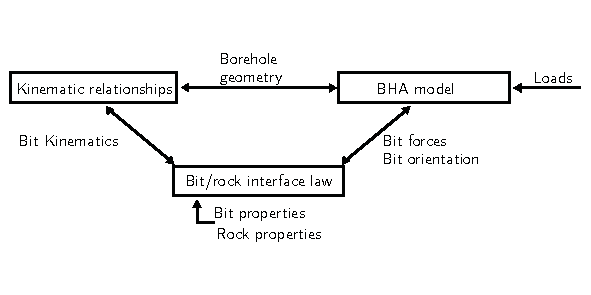
\includegraphics[width=0.6\textwidth]{img/modelinteraction.pdf}
	\caption{\label{fig:modelinter}Interaction between the elements of the model.}
\end{figure}

Furthermore, the vibrational effects in the BHA are ignored due to the fact that they take place at a much faster scale in time than the ones relevant for borehole propagation. This is why the forces and penetrations are averaged over several revolutions of the bit. An important consideration, is that the stabilizers are in constant  contact with the borehole wall, which in general is not always the case in practice. 

 The model is scaled at the BHA view by introducing two characteristic quantities:

\begin{align}
	L_* := \ell_1, \qquad F_* := \frac{3 E_y I}{\ell_1^2},
\end{align}

where $\ell_1$ is the distance between the bit and the first stabilizer (defining the characteristic length \lsymb{$L_*$}{Characteristic length in PD model.}) and the product of the Young's module \lsymb{$E_y$}{Young's module} with the area moment of inertia \lsymb{$I$}{Area moment of inertia.} represents the bending stiffness. The BHA is modeled as an Euler-Bernoulli beam, since deformations are presumed to be small because the radius of curvature of the borehole is large compared to $\ell_1$. The reason for $F_*$ being defined as shown, is that this is the reaction force induced at the end of a simply supported beam of length $\ell_1$ and stiffness $E_yI$ in response to a unit inclination angle imposed at the end. The characteristic length $L_*$ is used to scale the distance drilled $L$ into a dimensionless distance drilled $\xi$:

\begin{equation}
	\xi = \frac{L}{L_*}.
\end{equation}

\paragraph{BHA model.} Figure~\ref{fig:BHAmodel} shows the elements for a deflected BHA inside a borehole. The configuration is described by the position of the stabilizers and the RSS. Their location is given as $s = s_i$ where \lsymb{$s_i$}{Location of the i-th stablizer in PD model} is the $s$ coordinate of the i-th stablizer and $\Lambda \ell_1$ is the location of the RSS where $\Lambda \in [0,1]$. The distance between stabilizer $i$ and $i-1$ is given by \lsymb{$\ell_i$}{Length of BHA section i in PD model.} for $i = 2,...,n$ and $\ell_1$ defined as the distance between the bit and the first stabilizer again.

\begin{figure}[ht]\centering
	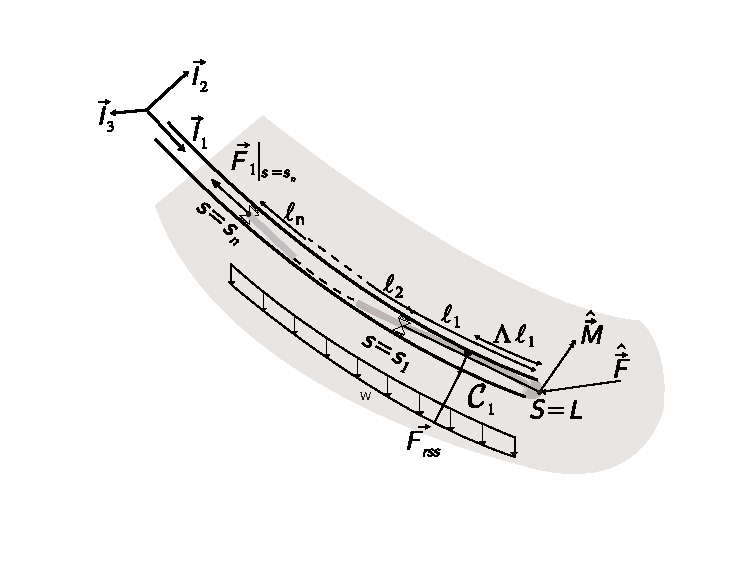
\includegraphics[width=0.4\textwidth]{img/BHAmodel.pdf}
	\caption{\label{fig:BHAmodel}Deflected BHA.}
\end{figure}

The external loads acting on the BHA are the distributed weight \lsymb{$\vec{w}$}{Distributed weight on the BHA for PD model.}, the RSS force \lsymb{$\vec{F}_{rss}$}{RSS force in the BHA for PD model.}, as well as the forces acting on the upper and lower boundaries of the BHA. The RSS force has two components over the $\vec{I}_2$ and $\vec{I}_3$ axes. These components along with the distributed weight are scaled using the characteristic force $F_*$ as:

\begin{align}
\Upsilon = \frac{w L_*}{F_*}, \qquad \Gamma_2 = \frac{F_{rss,2}}{F_*}, \qquad \Gamma_3 = \frac{F_{rss,3}}{F_*}.
\end{align}

In further derivations, uniform bending stiffness $E_y I$ and distributed weight $w$ for the BHA are assumed, the latter also being aligned with the chord \lsymb{$\mathcal{C}_1$}{Chord linking the bit and the first stabilizer.} which links the bit and the first stabilizer.

The governing equations for the transverse deflection of the BHA as an Euler-Bernoulli beam are:

\begin{align}
	E_y I \frac{\partial^3\theta_i}{\partial s^3} = w \sin{\langle \theta \rangle_1}, \qquad E_y I \sin{\langle \theta \rangle_1} \frac{\partial^3\phi_i}{\partial s^3} = 0,\label{eq:BHA}
\end{align}

where \lsymb{$\langle \theta \rangle_1$}{Inclination of chord $\mathcal{C}_1$ in PD model.} is the average inclination of the BHA between the bit and the first stabilizer. The BHA is divided in $n+1$ beams connected by constraints given for the previously established assumptions. Each section is modeled as a beam except for the one between the bit and the first stabilizer. This is separated into two parts, one corresponding to the section from the bit to the RSS and the other from the RSS to the first stabilizer. The equations for the whole profile can be written as:

\begin{align}
	\theta(\xi,s) &= \theta_{i}(\xi,s), \qquad \phi(\xi,s)= \phi_{i}(\xi,s), \qquad \kern0.1cm\textrm{ for } s \in [s_{i-1},s_{i}] \textrm{ for } i \in [2,...,n], \nonumber
	\\
	\theta(\xi,s) &= \theta_{1}(\xi,s), \qquad \phi(\xi,s)= \phi_{1}(\xi,s), \qquad \textrm{ for } s \in [\Lambda \ell_{1},s_{1}],
	\\
	\theta(\xi,s) &= \theta_{0}(\xi,s), \qquad \phi(\xi,s)= \phi_{0}(\xi,s), \qquad \textrm{ for } s \in [{0}, \Lambda \ell_{1}]. \nonumber
\end{align}

The general solution of Equation (\ref{eq:BHA}) holds:

\begin{align}
	\theta_{i}(\xi,s)&= \mathcal{A}_{i3} \left(\frac{s}{\ell_1}\right)^3 + \mathcal{A}_{i2}\left(\frac{s}{\ell_1}\right)^2+ \mathcal{A}_{i1}\left(\frac{s}{\ell_1}\right) + \mathcal{A}_{i0},
	\nonumber \\
	\phi_{i}(\xi,s)&= \mathcal{B}_{i2}\left(\frac{s}{\ell_1}\right)^2+ \mathcal{B}_{i1}\left(\frac{s}{\ell_1}\right) + \mathcal{B}_{i0}. \label{eq:solutionBHA}
\end{align}

To obtain the coefficients in (\ref{eq:solutionBHA}), a set of $6(n+1)$ constraints needs to be imposed depending on factors related to the previously mentioned assumptions and features of the BHA. These constraints and coefficients \lsymb{$\mathcal{A}_{ij}$}{Coefficients of inclination angle for general solution of BHA profile in PD model.} and \lsymb{$\mathcal{B}_{ij}$}{Coefficients of azimuth angle for general solution of BHA profile in PD model.} are explained in detail at~\cite{Monsieurs2015} in the case of two stabilizers. Finally the expressions for shear forces and bending moments acting on the bit expressed in the bit basis are obtained as:

\begin{align}
	\frac{{{{\hat F}_2}}}{{{F_*}}} &= {\mathcal{F}_b}\left( {\hat \theta  - {{\rm{\langle\Theta }}\rangle}_1} \right)+{\mathcal{F}_w}\Upsilon \sin {{\rm{\langle\Theta\rangle }}_1} + {\mathcal{F}_r}{\Gamma _2} + \mathop \sum \limits_{i = 1}^{n - 1} {\mathcal{F}_i}\left( {{{\rm{\langle\Theta\rangle }}_i} - {{\rm{\langle\Theta\rangle }}_{i + 1}}} \right),
	\nonumber \\
	\frac{{{{\hat M}_3}}}{{{F_*}{\ell _1}}} &= {\mathcal{M}_b}\left( {\hat \theta  - {{\rm{\langle\Theta\rangle }}_1}} \right) + {\mathcal{M}_w}\Upsilon \sin {{\rm{\langle\Theta\rangle }}_1} + {\mathcal{M}_r}{\Gamma _2} + \mathop \sum \limits_{i = 1}^{n - 1} {\mathcal{M}_i}\left( {{{\rm{\langle\Theta\rangle }}_i} - {{\rm{\langle\Theta\rangle }}_{i + 1}}} \right),
	\nonumber \\
	\frac{{{{\hat F}_3}}}{{{F_*}}} &= {\mathcal{F}_b}\left( {\hat \phi  - {\langle\Phi \rangle}_1} \right)\sin {{\rm{\langle\Theta\rangle }}_1} + {\mathcal{F}_r}{\Gamma _3} + \mathop \sum \limits_{i = 1}^{n - 1} {\mathcal{F}_i}\left( {{{\rm{\langle\Phi\rangle }}_{\rm{i}}} - {{\rm{\langle\Phi\rangle }}_{{\rm{i}} + 1}}} \right)\sin {{\rm{\langle\Theta }}\rangle_1},
	\nonumber \\
	\frac{{{{\hat M}_2}}}{{{F_*}{\ell _1}}} &=  - {\mathcal{M}_b}\left( {\hat \phi  - \langle{\Phi }\rangle_1} \right)\sin {{\rm{\langle\Theta\rangle }}_1} - {\mathcal{M}_r}{\Gamma _3} - \mathop \sum \limits_{i = 1}^{n - 1} {\mathcal{M}_i}\left( {{{\rm{\langle\Phi\rangle }}_i} - {{\rm{\langle\Phi\rangle }}_{i + 1}}} \right)\sin {{\rm{\langle\Theta\rangle }}_1},
	\label{eq:BHAforcemomentequations}
\end{align}

where \lsymb{$\mathcal{F}_{b}$, $\mathcal{F}_{r}$, $\mathcal{F}_{w}$, $\mathcal{F}_{i}$}{Coefficients related to force influence in PD model.}, \lsymb{$\mathcal{M}_{b}$, $\mathcal{M}_{r}$, $\mathcal{M}_{w}$, $\mathcal{M}_{i}$}{Coefficients related to moment influence in PD model.} are constant coefficients for a given BHA configuration which can be found in~\cite{Monsieurs2015}, and the average borehole inclination and azimuth at the i-th stabilizer \gsymb{${\rm{\langle\Theta }}\rangle_i$}{Average borehole inclination of i-th stabilizer.} and \gsymb{${\rm{\langle\Phi }}\rangle_i$}{Average borehole azimuth of i-th stabilizer.} are given by:

\begin{equation}
	{{\rm{\langle\Theta\rangle }}_i}:= \frac{1}{\varkappa_i}\int \limits_{\xi_{i-1}}^{\xi_i} \Theta(\sigma)d\sigma, \qquad
	{{\rm{\langle\Phi\rangle }}_i}:=\frac{1}{\varkappa_i}\int \limits_{\xi_{i-1}}^{\xi_i} \Phi(\sigma)d\sigma
	\label{eq:definitionaveragestates},
\end{equation}

where \gsymb{$\varkappa_i$}{Dimensionless length of i-th section in PD model.} is the dimensionless length of the i-th section given by $\varkappa_i = \frac{\ell_i}{\ell_1}$ and \gsymb{$\xi_i$}{Dimensionless position of stabilizer $i$.} is the dimensionless position of stabilizer $i$.

\paragraph{Kinematic relationships.} The motion of the bit is described by the linear velocity vector \lsymb{$\vec{v}$}{Linear velocity of the bit in PD/Neubert and Heisig models.}, the spin vector \gsymb{$\vec{\omega}$}{Spin vector of the bit in PD model.} and the angular velocity \gsymb{$\vec{\Omega}$}{Angular velocity vector of the bit in PD/Neuber and Heisig models.}. The bit is rotating around $\vec{i}_1$ with angular velocity $\vec{\Omega}$. Using this we can define the two main penetration variables:

\begin{align}
	\vec{d} := \frac{2 \pi \vec{v}}{|\vec{\Omega}|}, \qquad \vec{\varphi} := \frac{2 \pi \vec{\omega}}{|\vec{\Omega}|}
	\label{eq:penetrationvectors},
\end{align}

where \lsymb{$\vec{d}$}{Linear penetration in PD/Neubert and Heisig models.} and \lsymb{$\vec{\varphi}$}{Angular penetration in PD model.} are the linear and angular penetration respectively. The linear penetration is the increment of the borehole over one revolution, which is expressed by using the operator $\delta(.) = |\vec{d}|\frac{d(.)}{dL}$. With this definition, the magnitude of the linear penetration $d = |\vec{d}|$ is equal to the increment of the borehole length $\delta L$.

The two penetration variables are decomposed in five quantities corresponding to $\vec{d}=d_1\hat{\vec{i}}_1+d_2\hat{\vec{i}}_2+d_3\hat{\vec{i}}_3$ as well as $\varphi_2$ and $\varphi_3$ as the rotations around vectors $\hat{\vec{i}}_2$ and $\hat{\vec{i}}_3$ respectively. It is assumed that $d_1 \approx |\vec{d}|$ because components $d_2$ and $d_3$ depend on the tilt angles $\psi_2$ and $\psi_3$ which are generally small under normal drilling conditions and defined by:

\begin{align}
	{d_2} &= -\psi_{2} d_1, \nonumber \\ 
	{d_3} &= -\psi_{3} d_{1}.
	\label{eq:vector_d}
\end{align}

In addition, the expressions for $\varphi_2$ and $\varphi_3$ are given as:

\begin{align}
	{\varphi_2} &= - \frac{d_{1}}{\ell_1} \frac{d\hat\phi}{d\xi}\sin\hat\theta, \nonumber \\
	{\varphi_3} &= \frac{d_{1}}{\ell_1} \frac{d\hat\theta}{d\xi},
	\label{eq:vector_phi}
\end{align}

where these expressions are obtained by projecting the cross product $\hat{\vec{i}}_1 \times \delta \hat{\vec{i}}_1$ onto the bit basis.

\paragraph{Bit/rock interface law.} This element of the model represents the interaction between the kinematics of the bit and both the forces and moments reacting on the bit due to the properties of the drilled surface. The complete deduction of this interaction law is given in~\cite{Perneder2013}, which arrives to the following expression in the three-dimensional case:

\begin{equation}
\begin{bmatrix}
\frac{{{{\hat F}_2}}}{{{F_*}}}    \\
\frac{{{{\hat F}_3}}}{{{F_*}}}       \\
\frac{{{{\hat M}_2}}}{{{F_*}}\ell_1}    \\
\frac{{{{\hat M}_3}}}{{{F_*}}\ell_1}       \\
\end{bmatrix}
=
\begin{bmatrix}
{\eta\Pi}\cos \varpi       & {\eta\Pi}\sin \varpi  & 0 & 0    \\
-{\eta\Pi}\sin \varpi      & {\eta\Pi}\cos \varpi   & 0 & 0     \\
0      & 0  & -\frac{\chi\Pi\ell_1}{d_1} & 0     \\
0      & 0  & 0 & -\frac{\chi\Pi\ell_1}{d_1}     \\
\end{bmatrix}
\begin{bmatrix}
\frac{d_2}{d_1}\\
\frac{d_3}{d_1} \\
\varphi_2 \\
\varphi_3 \\
\end{bmatrix},
\label{eq:bitrockdimensionless}
\end{equation}

where the newly introduced parameters \gsymb{$\eta$}{Lateral steering resistance in PD model.}, \gsymb{$\chi$}{Angular steering resistance in PD model.}, \gsymb{$\varpi$}{Bit walk angle in PD model.} and \gsymb{$\Pi$}{Active weight on bit in PD model.} are the lateral steering resistance, the angular steering resistance, the bit walk angle and the active weight on bit. The first two come from the inherent properties of the rock and the cutter geometry. In the case of the latter two, they are not known exactly during the drilling process and usually taken to be uncertain.

\paragraph{Borehole evolution equations.} After combining the BHA model Equations (\ref{eq:BHAforcemomentequations}), the kinematic relationships (\ref{eq:vector_d}) and (\ref{eq:vector_phi}) and the bit/rock interface law (\ref{eq:bitrockdimensionless}), the borehole evolution equations are derived as:


	\begin{align}
	&\eta \Pi \Big((\theta-\Theta) \cos{\varpi}+\sin \Theta\sin{\varpi} \left( {\phi  - \Phi } \right)\Big)=\mathcal{F}_b\left( {\theta  - {{\rm{\langle\Theta\rangle }}_1}} \right)+{\mathcal{F}_w}\Upsilon \sin{{\rm{\langle\Theta\rangle }}_1}+{\mathcal{F}_r}{\Gamma _2} \nonumber
	\\
	&\kern6.65cm+ \mathop \sum \limits_{i = 1}^{n - 1} {\mathcal{F}_i}\left( {{{\rm{\langle\Theta\rangle }}_i} - {{\rm{\langle\Theta\rangle }}_{i + 1}}} \right), \label{eq:inc_con}
	\\
	&- \chi \Pi \theta {\rm{'}} = \mathcal{M}_b\left( {\theta  - {{\rm{\langle\Theta\rangle }}_1}} \right) + {\mathcal{M}_w}\Upsilon \sin {{\rm{\langle\Theta\rangle }}_1} + {\mathcal{M}_r}{\Gamma _2} + \mathop \sum \limits_{i = 1}^{n - 1} {\mathcal{M}_i}\left( {{{\rm{\langle\Theta\rangle }}_i} - {{\rm{\langle\Theta\rangle }}_{i + 1}}} \right), \label{eq:inc_dde}
	\\ \nonumber
	&\eta \Pi \Big(-(\theta-\Theta) \sin{\varpi}+\cos{\varpi}\sin \Theta \left( {\phi  - \Phi } \right)\Big)= \mathcal{F}_b\left( {\phi  - {{\rm{\langle\Phi\rangle }}_1}} \right)\sin {{\rm{\langle\Theta\rangle }}_1} + {\mathcal{F}_r}{\Gamma _3} \nonumber
	\\
	&\kern7.1cm+ \mathop \sum \limits_{i = 1}^{n - 1} {\mathcal{F}_i}\left( {{{\rm{\langle\Phi\rangle }}_i} - {{\rm{\langle\Phi\rangle }}_{i + 1}}} \right)\sin {{\rm{\langle\Theta\rangle }}_1}, \label{eq:azi_con}
	\\
	&- \chi \Pi \phi '\sin \theta  = \mathcal{M}_b\left( {\phi  - {{\rm{\langle\Phi\rangle }}_1}} \right)\sin {{\rm{\langle\Theta\rangle }}_1} + {\mathcal{M}_r}{\Gamma _3} + \mathop \sum \limits_{i = 1}^{n - 1} {\mathcal{M}_i}\left( {{{\rm{\langle\Phi\rangle }}_i} - {{\rm{\langle\Phi\rangle }}_{i + 1}}} \right)\sin {{\rm{\langle\Theta\rangle }}_1}. \label{eq:azi_dde}
	\end{align}

This set of equations represents the way the borehole will evolve along the independent variable $\xi$ and with respect to the borehole and BHA inclination and azimuth. As the important variables for control are only the ones related to the borehole, in~\cite{Monsieurs2015} explicit expressions for the borehole inclination and azimuth derivatives were obtained. These are:

\begin{equation}
	\mathcal{E} \begin{bmatrix}
	{\Theta'}\\
	{\Phi'}
	\end{bmatrix}
	=
	\begin{bmatrix}\begin{aligned}
	&- \frac{1}{{\chi \Pi }}\bigg(\mathcal{M}_b\left(\frac{{a_1} + {a_2}{a_3}}{1-{a_2}{a_4}}-{{\rm{\langle\Theta\rangle }}_1}\right)+{\mathcal{M}_w}\Upsilon \sin {{\rm{\langle\Theta\rangle }}_1} + {\mathcal{M}_r}{\Gamma _2}+...
	\\
	&\kern5.9cm+ \mathop \sum \limits_{i = 1}^{n - 1} {\mathcal{M}_i}\left( {{{\rm{\langle\Theta\rangle }}_i} - {{\rm{\langle\Theta\rangle }}_{i + 1}}} \right)\bigg) - \frac{b_3+a_2b_7}{1-a_2a_4}   \\
	&- \frac{1}{{\chi \Pi }}\bigg(\mathcal{M}_b\left(\frac{a_3+a_4a_1}{1-a_4a_2 }-{{\rm{\langle\Phi\rangle }}_1}\right)+ {\mathcal{M}_r}\frac{\Gamma _3}{\sin\Theta}+...
	\\
	&\kern5.9cm+ \mathop \sum \limits_{i = 1}^{n - 1} {\mathcal{M}_i}\left( {{{\rm{\langle\Phi\rangle }}_i} - {{\rm{\langle\Phi\rangle }}_{i + 1}}} \right)\bigg)
	-\frac{a_4b_3+b_7}{1-a_2a_4}
	\end{aligned}\end{bmatrix},
	\label{eq:finalmodel}
\end{equation}

where $\mathcal{E}$ is given by:

\begin{equation}
\mathcal{E} = \frac{1}{1-a_2a_4}
	\begin{bmatrix}
	b_1 + a_3b_4 + a_2b_5 +\frac{(a_1+a_2a_3)(a_4b_4+a_2b_8)}{1-a_2a_4} & \qquad b_2+a_2b_6\\
	a_4b_1 + b_5 + a_1b_8 +\frac{(a_3+a_4a_1)(a_4b_4+a_2b_8)}{1-a_2a_4} & \qquad a_4b_2+b_6 \\
	\end{bmatrix},
\end{equation}

and the coefficients \lsymb{$a_i$}{Auxiliary variables for BHA orientation dependency elimination in PD model.} are auxiliary variables to eliminate the dependency to the BHA orientation in the borehole evolution equations and \lsymb{$b_i$}{Auxiliary variables for BHA orientation derivative dependency elimination in PD model.} are used to eliminate the dependency on the derivative of the orientation of the BHA. The detailed derivation of this coefficients is given in~\cite{Monsieurs2015}. This set of equations can be classified as nonlinear delay differential equations. 

It can be seen that this model has several advantages with respect to the other ones presented in this section. It possesses a detailed bit/rock interaction model and it also captures the delayed nature of the process. Furthermore, the model is developed for a three-dimensional system. It can also be said, that a convenient state-space representation has been worked out in order to develop controllers in~\cite{Monsieurs2015}. Despite this advantages, as most of the models developed up to this point, it lacks the inclusion of nonlinear effects such as bit-tilt saturation and relies on assumptions such as contacts with the stabilizers. 

\subsection{Discussion}

It is clear that the models presented in this chapter have very important differences. First of all, regarding numerical and input/output correlation models, despite its usefulness in the past to predict trajectories and estimate the behavior of the system, its complexity and lack of generality makes them non-suitable for controller design, which is ultimately the goal of this research. 

One of the key aspects that has to be taken into account is the dimension of the space in which they are modeled in. Excluding the EFFSZM model, the descriptions used to design controllers were performed for a three-dimensional movement. This is important, since the borehole spiraling is inherently a 3D effect~\cite{Marck2015} and one of the main issues regarding control is the reduction of this unwanted behavior.

Another important aspect, is how detailed the models are. In the case of the kinematic models presented here, the effects of forces are not taken into account, opposite to the other three models. It would be interesting to prove if the influence of these is truly significant in the borehole evolution, by doing a comparison of the response for all models under similar conditions. Furthermore, since no forces are being considered in the kinematic model, the control inputs are given in terms of angles, which is clearly a disadvantage because the RSS input is explicitly force.

Regarding the effect of forces as well, from the three models that do take them into account, only the Neubert and Heisig and the PD model have a detailed rock/bit interaction model. This is relevant because the bit walk angle becomes present from this interaction, which obviously is not present in the EFFSZM model because it is a 2D model.

A big drawback on the EFFSZM is that it only provides a description in terms of deflection for small rotation angles around an initial borehole/BHA orientation. This disadvantage is not present in the PD model, where the magnitude of the rotation angles is not limitation for the model.

As for the usefulness for control, the EFFSZM and the PD model have explicit expressions, in transfer function and state-space form, respectively, which are convenient ways to start developing algorithms. Neubert and Heisig have developed a controller in~\cite{Neub97}, but it is difficult to find an international publication with a detailed description of it.

It is clear that in control, an essential aspect is where the measurement of the states is coming from. Kinematic models assumed the measurement coming from non-spatially coincidental sensors at the bit, which in most cases are dealt with using some kind of time delay compensation. In the case of the EFFSZM model, there is no difference between the spatial difference of the measurement and the bit. Looking at the PD model derived in~\cite{Monsieurs2015}, the output equations do take into account sensor positioning.

An important feature of the models, is to check whether they have been validated in some way. In the case of EFFSZM there exist some publications~\cite{Down07} where the data is compared with the previously mentioned ST2 model. The PD model has been compared to some field data in~\cite{Marck2015} providing a good match for the description of the model. 

It seems after this initial outline of the models, that the model which is most suitable at the time for controller is the PD model, since it takes into account important elements presents in the directional drilling process. Furthermore, the fact that work has been done to develop output-feedback controllers has lead to a convenient state-space representation to start assessing new challenges for the process.

\end{document}

